% !TeX spellcheck = en_GB
% !TeX root = ../../build/architecture.tex

\section{Simple Virtual Machine}

\begin{frame}{Main State Machine of a Simplified Virtual Machine}
\begin{figure}
	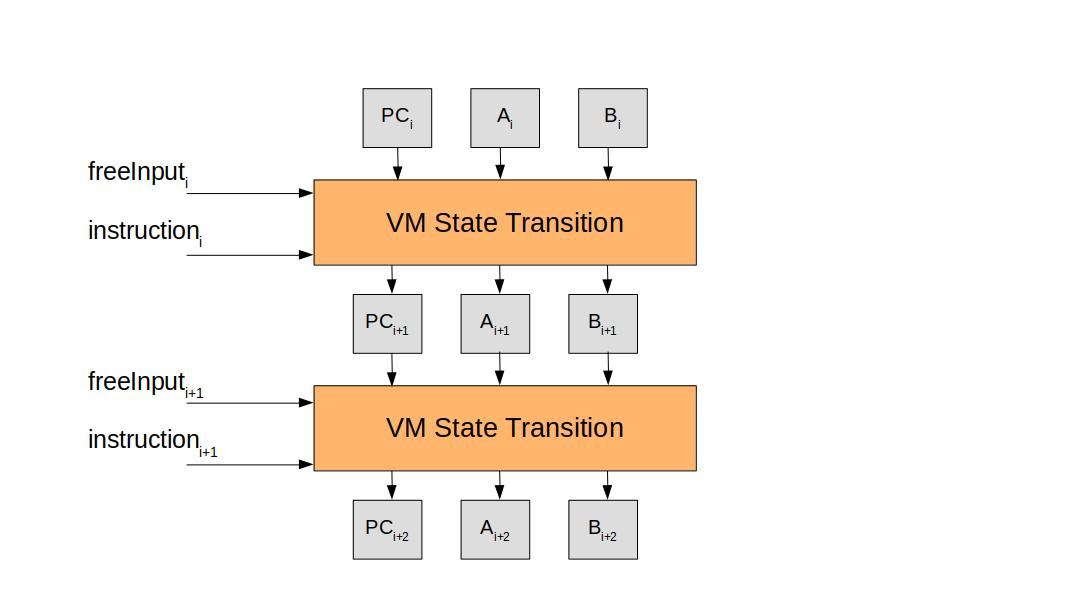
\includegraphics[width=0.65\textwidth]{\zkevmdir/architecture/figures/main-state-machine-simplified-overview}
\end{figure}
\end{frame}









\begin{frame}[allowframebreaks]{Example Program: Moving \& Jumping}
\begin{itemize}
\item Let's assume we have the following program:
\[
\begin{array}{|c|l|c|}
\hline
\mathbf{Position} & \multicolumn{2}{|c|}{\mathbf{Instruction}} \\ \hline
0 & \mathbf{MOV} & A, 7 \\ \hline
1 & \mathbf{JMP}~(if~A = 0) & 5 \\ \hline
2 & \mathbf{MOV} & B, 3 \\ \hline
3 & \mathbf{MOV} & A, 0 \\ \hline
4 & \mathbf{JMP} & 1 \\ \hline
5 & \mathbf{STOP} & \emptyset \\ \hline
\end{array}
\]

\item This program has the following trace:
\[
\begin{array}{|c|l|c|c|c|c|c|c|c|}
\hline
\mathbf{Position} & \multicolumn{2}{|c|}{\mathbf{Instruction}} & \mathbf{PC_i} & \mathbf{A_i} & \mathbf{B_i} & \mathbf{PC_{i+1}} & \mathbf{A_{i+1}} & \mathbf{B_{i+1}} \\ \hline
0 & \mathbf{MOV} & A, 7 & 0 & 0 & 0 & 1 & 7 & 0 \\ \hline
1 & \mathbf{JMP}~(if~A = 0) & 5 & 1 & 7 & 0 & 2 & 7 & 0 \\ \hline
2 & \mathbf{MOV} & B, 3 & 2 & 7 & 0 & 3 & 7 & 3 \\ \hline
3 & \mathbf{MOV} & A, 0 & 3 & 7 & 3 & 4 & 0 & 3 \\ \hline
4 & \mathbf{JMP} & 1 & 4 & 0 & 3 & 1 & 0 & 3 \\ \hline
5 & \mathbf{JMP}~(if~A = 0) & 5 & 1 & 0 & 3 & 5 & 0 & 3 \\ \hline
6 & \mathbf{STOP} & \emptyset & 5 & 0 & 3 & 5 & 0 & 3 \\ \hline
\end{array}
\]
\end{itemize}
\end{frame}






\begin{frame}[allowframebreaks]{Expressing the Relations between the States}
\vspace{-0.3cm}
\begin{figure}
	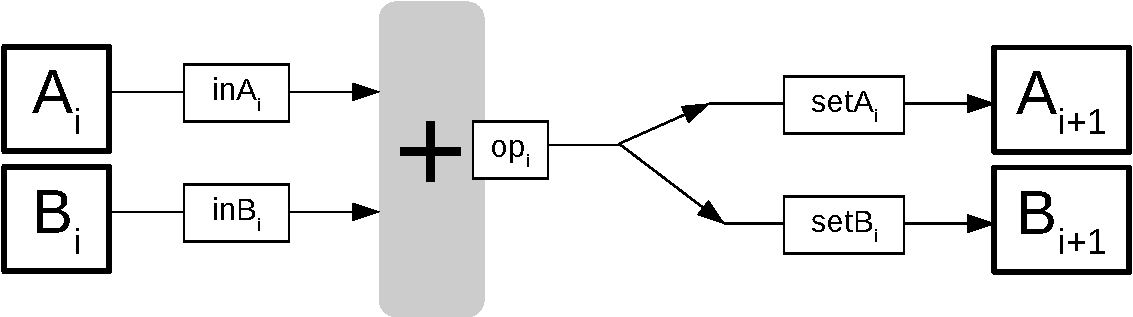
\includegraphics[width=0.8\textwidth]{\zkevmdir/architecture/figures/main-state-machine-2registres}
\end{figure}

\begin{itemize}
\item Here, we use the following notation:
\begin{enumerate}[a)]
\item $\mathbf{inX_i}$: $1$ or $0$ depending if the state $X_i$ is included in the sum or not.

\item $\mathbf{op_i}$: The resulting operation between the included states.

\item $\mathbf{setX_i}$: $1$ or $0$ depending if $\op_i$ will be moved into $X_{i+1}$.
\end{enumerate}
 
\item The relations between the states of the registries can be expressed as follows:
\begin{align*}
\op_i &= A_i \cdot \inp A_i + B_i \cdot \inp B_i + FREE_i \cdot \inp FREE_i, \\
A_{i+1} &= \set A_i \cdot (\op_i - A_i) %+ freeload_i \cdot (value - A_i) 
+ A_i, \\
B_{i+1} &= \set B_i \cdot (\op_i - B_i) %+ freeload_i \cdot (value - B_i) 
+ B_i, \\
PC_{i+1} &= PC_i + 1 + (isJMP_i + isJMPC_i \cdot isSatisfied_i) \cdot (dest - PC_i - 1).
\end{align*}

\item Here:
\begin{enumerate}
\item $FREE$ is the second input passed to the \textbf{MOV} instruction.
%\item $value$ is the input passed to the FREELOAD instruction.

\item $dest$ is the input passed to the \textbf{JMP} or the \textbf{JMPC} (conditioned) instructions.
\end{enumerate}
\end{itemize}
\end{frame}










\begin{frame}[allowframebreaks]{How to Encode the Move State Machine}
\begin{itemize}
\item Let's now explain how to encode the instructions included in the program:
\begin{align*}
\mathbf{MOV}~A, 7 \quad \mathbf{JMP}~(if~A = 0)~5 \quad \mathbf{MOV}~B,3 \quad \mathbf{MOV}~A,0 \quad \mathbf{JMP}~1 \quad \mathbf{STOP}
\end{align*}
\end{itemize}
\[
\scriptsize
\begin{array}{|c|c|}
\hline
\multicolumn{2}{|c|}{\mathbf{Instruction}} \\ \hline
\mathbf{MOV} & A, 7 \\ \hline
\mathbf{JMP}~(if~A = 0) & 5 \\ \hline
\mathbf{MOV} & B,3 \\ \hline
\mathbf{JMP} & 1 \\ \hline
\mathbf{STOP} & \emptyset \\ \hline
\end{array}
\hspace{0.1cm}
\begin{array}{|c|c|c|c|c|c|c|c|}
\hline
\textbf{inA} & \textbf{inB} & \textbf{inFREE} & \textbf{setA} & \textbf{setB} & \textbf{isJMP} & \textbf{isJMPC} \\ \hline
1 & 0 & 1 & 1 & 0 & 0 & 0 \\ \hline
0 & 0 & 0 & 0 & 0 & 0 & 1 \\ \hline
0 & 1 & 1 & 1 & 0 & 0 & 0 \\ \hline
0 & 0 & 0 & 0 & 0 & 0 & 1  \\ \hline
0 & 0 & 0 & 0 & 0 & 0 & 0 \\ \hline
\end{array}
\hspace{0.1cm}
\begin{array}{|c|c|}
\hline
\mathbf{FREE} & \mathbf{dest} \\ \hline
7 & 0 \\ \hline
0 & 5 \\ \hline
3 & 0 \\ \hline
0 & 1 \\ \hline
0 & 0 \\ \hline
\end{array}
\hspace{0.1cm}
\begin{array}{|c|}
\hline
\mathbf{Inst.~Value} \\ \hline
0000.0111.0001101 \\ \hline
0101.0000.1000000 \\ \hline
0000.0011.0001110 \\ \hline
0001.0000.1000000 \\ \hline
0000.0000.0000000 \\ \hline
\end{array}
\]

\normalsize
\begin{itemize}
\item Here, we computed the instruction values as follows:
\begin{align*}
\mathsf{inst}_i = &~\inp A_i + 2 \cdot \inp B_i + 2^2 \cdot \inp FREE_i + 2^3 \cdot \set A_i + 2^4 \cdot \set B_i + 2^5 \cdot isJMP_i + 2^6 \cdot isJMPC_i \\ 
& + 2^{10} \cdot FREE_i + 2^{14} \cdot dest_i.
\end{align*}

\item We can write the previous table values as the following polynomial identity:
\begin{align*}
\mathsf{inst}(x) = &~\inp A(x) + 2 \cdot \inp B(x) + 2^2 \cdot \inp FREE(x) + 2^3 \cdot \set A(x) + 2^4 \cdot \set B(x) + 2^5 \cdot isJMP(x) \\
& + 2^6 \cdot isJMPC(x) + 2^{10} \cdot FREE(x) + 2^{14} \cdot dest(x).
\end{align*}

\item Now, to build the program, every instruction will be uniquely identified by its value and the position of the program in which it is executed.

\item We define the polynomial $\mathsf{rom}(x)$ which consists on an instruction value concatenated with its position:
\[
\mathsf{rom}(x) = \mathsf{inst}(x) + 2^{18} \cdot position(x)
\]
\end{itemize}
\end{frame}










\begin{frame}[allowframebreaks]{Representing the State Machine}
\begin{itemize}
\item With the support of this encoding, now we can compute the whole trace of the execution of this program:
\[
\begin{array}{|c|l|c|c|}
\hline
\mathbf{Position} & \multicolumn{2}{|c|}{\mathbf{Instruction}} \\ \hline
0 & \mathbf{MOV} & A, 7 \\ \hline
1 & \mathbf{JMP}~(if~A = 0) & 5 \\ \hline
2 & \mathbf{MOV} & B, 3 \\ \hline
3 & \mathbf{MOV} & A, 0 \\ \hline
4 & \mathbf{JMP} & 1 \\ \hline
5 & \mathbf{STOP} & \emptyset \\ \hline
\end{array}
\hspace{0.1cm}
\begin{array}{|c|c|}
\hline
\mathbf{Rom} = inst(x) + 2^{19} \cdot position(x) \\ \hline
0000.0000.0111.0001101 \\ \hline
0001.0101.0000.1000000 \\ \hline
0010.0000.0011.0001110 \\ \hline
0011.0000.0000.0001101 \\ \hline
0100.0001.0000.1000000 \\ \hline
0101.0000.0000.0000000 \\ \hline
\end{array}
\]

\item We can do the same with the trace of the program:
\[
\begin{array}{|c|l|c|c|c|c|}
\hline
\mathbf{Position} & \multicolumn{2}{|c|}{\mathbf{Instruction}} & \mathbf{PC_i} & \mathbf{A_i} & \mathbf{B_i} \\ \hline
0 & \mathbf{MOV} & A, 7 & 0 & 0 & 0 \\ \hline
1 & \mathbf{JMP}~(if~A = 0) & 5 & 1 & 7 & 0 \\ \hline
2 & \mathbf{MOV} & B, 3 & 2 & 7 & 0 \\ \hline
3 & \mathbf{MOV} & A, 0 & 3 & 7 & 3 \\ \hline
4 & \mathbf{JMP} & 1 & 4 & 0 & 3 \\ \hline
5 & \mathbf{JMP}~(if~A = 0) & 5 & 1 & 0 & 3 \\ \hline
6 & \mathbf{STOP} & \emptyset & 5 & 0 & 3 \\ \hline
\end{array}
\hspace{0.1cm}
\begin{array}{|c|c|}
\hline
\mathbf{instTrace} = inst(x) + 2^{19} \cdot PC(x) \\ \hline
0000.0000.0111.0001101 \\ \hline
0001.0101.0000.1000000 \\ \hline
0010.0000.0011.0001110 \\ \hline
0011.0000.0000.0001101 \\ \hline
0100.0001.0000.1000000 \\ \hline
0001.0101.0000.1000000 \\ \hline
0000.0000.0000.0000000 \\ \hline
\end{array}
\]
\end{itemize}
\end{frame}












\begin{frame}[allowframebreaks]{Checking the Correct Program Execution}
\begin{itemize}
\item The question that arises now is:
\begin{center}
\textbf{How do we actually verify that we are executing the correct program?}
\end{center}

\item The solution seems obvious: Check that every row of the trace of the execution coincides with some row of the program.

\item Then, the question becomes to:
\begin{center}
\textbf{How do we actually verify that we are executing the correct program \\ in an efficient manner?}
\end{center}

\framebreak

\item We can do it with the Plookup protocol!

\item So, to check that the correct program is being executed, we simply have to use Plookup to determine if:
\[
\mathbf{instTrace} \subset \mathbf{Rom}
\]

\item In simple words, the trace being executed is an execution of the actual program if the instruction trace is contained in the ROM of the program.
\end{itemize}
\end{frame}











\begin{frame}{Strategy to Follow}
\begin{itemize}
\item The strategy to follow to check the correct execution of a program is:
\begin{enumerate}
\item Encode each distinct instruction of the program in a deterministic and efficient manner.

\item Represent each instruction in the program in a unique manner by appending the position in the program to it. We obtain the polynomial $rom(x)$.

\item Similarly, represent each instruction in the trace of the program by appending the program counter to it.We obtain the polynomial $instTrace(x)$.

\item Use Plookup to prove that the trace of the program is contained in the rom of the program, i.e., prove that $instTrace \subset rom$.
\end{enumerate}
\end{itemize}
\end{frame}








%\begin{frame}{Example Program}
%\begin{itemize}
%\item Let's assume we have the following program:
%\[
%\begin{array}{|c|l|c|}
%\hline
%\mathbf{Position} & \multicolumn{2}{|c|}{\mathbf{Instruction}} \\ \hline
%0 & \mathbf{MOV} & A, 10 \\ \hline
%1 & \mathbf{MOV} & B, 3 \\ \hline
%2 & \mathbf{JMP}~(if~B = 0) & 6 \\ \hline
%3 & \mathbf{MUL} & A, A \\ \hline
%4 & \mathbf{DEC} & B \\ \hline
%5 & \mathbf{JMP} & 2 \\ \hline
%6 & \mathbf{STOP} & \emptyset \\ \hline
%\end{array}
%\]
%\end{itemize}
%\end{frame}







%TODO: Do it step by step (limiting only moving one state to another and blabla) and better explanations

%TODO: Generalize it to multiple states in parallel
%\begin{frame}[allowframebreaks]{Starting from the Basics: Move State Machine}
%\vspace{-0.3cm}
%\begin{figure}
%	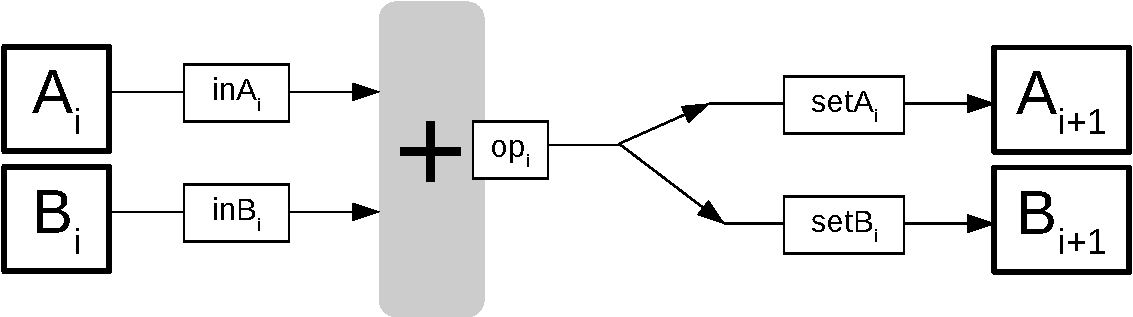
\includegraphics[width=0.8\textwidth]{\zkevmdir/architecture/figures/main-state-machine-2registres}
%\end{figure}
%
%\begin{itemize}
%\item We have used the following notation:
%\begin{enumerate}[a)]
%\item \textbf{inX}: $1$ or $0$ depending if the state $X_i$ is included in the sum or not.
%
%\item \textbf{op}: The resulting operation between the included states.
%
%\item \textbf{setX}: $1$ or $0$ depending if one state (or a combination or more) will be moved into $X_{i+1}$.
%\end{enumerate}
% 
%\item The relations between the states of the registries can be expressed as follows:
%\begin{align*}
%\op_i &= A_i \cdot \inp A_i + B_i \cdot \inp B_i + FREE_i \cdot \inp FREE_i, \\
%aux_i &= \op_i +  isM_i \cdot \op_i \cdot (\op_i - 1) \\
%A_{i+1} &= \set A_i \cdot (aux_i - A_i) %+ freeload_i \cdot (value - A_i) 
%+ A_i - dec_i, \\
%B_{i+1} &= \set B_i \cdot (aux_i - B_i) %+ freeload_i \cdot (value - B_i) 
%+ B_i - dec_i, \\
%PC_{i+1} &= PC_i + 1 + isJMP \cdot (dest - PC_i - 1) + isJMPC \cdot (isSatisfied_i \cdot (dest - PC_i - 1)).
%\end{align*}
%
%\item Here:
%\begin{enumerate}
%\item $FREE$ is the second input passed to the MOV function.
%%\item $value$ is the input passed to the FREELOAD instruction.
%
%\item $dest$ is the input passed to the JMP or the conditioned JMP instructions.
%\end{enumerate}
%\end{itemize}
%\end{frame}
%
%
%
%
%
%
%
%\begin{frame}[allowframebreaks]{How to Encode the Move State Machine}
%\begin{itemize}
%\item Let's now explain how to encode the instructions included in the program:
%\begin{align*}
%\mathbf{MOV}~A, 10 \quad \mathbf{MOV}~B, 3 \quad \mathbf{JMP}~2 \quad \mathbf{JMP}~(if~B = 0)~6 \quad \mathbf{MUL}~A, A \quad \mathbf{DEC}~B \quad \mathbf{STOP}
%\end{align*}
%\end{itemize}
%\small
%%TODO: Add dest and FREE
%\[
%\begin{array}{|c|c|}
%\hline
%\multicolumn{2}{|c|}{\mathbf{Instruction}} \\ \hline
%\mathbf{MOV} & A, 10 \\ \hline
%\mathbf{MOV} & B, 3 \\ \hline
%\mathbf{JMP} & 2 \\ \hline
%\mathbf{JMPC} & 6 \\ \hline
%\mathbf{MULT} & A, A \\ \hline
%\mathbf{DEC} & B \\ \hline
%\mathbf{STOP} & \emptyset \\ \hline
%\end{array}
%\hspace{0.1cm}
%\begin{array}{|c|c|c|c|c|c|c|c|c|}
%\hline
%\textbf{inA} & \textbf{inB} & \textbf{dec} & \textbf{inFREE} & \textbf{setA} & \textbf{setB} & \textbf{isJMP} & \textbf{isJMPC} & \textbf{isMULT} \\ \hline
%0 & 0 & 0 & 1 & 1 & 0 & 0 & 0 & 0 \\ \hline
%0 & 0 & 0 & 1 & 0 & 1 & 0 & 0 & 0 \\ \hline
%0 & 0 & 0 & 0 & 0 & 0 & 1 & 0 & 0 \\ \hline
%0 & 0 & 0 & 0 & 0 & 0 & 0 & 1 & 0 \\ \hline
%1 & 0 & 0 & 0 & 0 & 0 & 0 & 0 & 1 \\ \hline
%0 & 1 & 1 & 0 & 0 & 0 & 0 & 0 & 0 \\ \hline
%0 & 0 & 0 & 0 & 0 & 0 & 0 & 0 & 0 \\ \hline
%\end{array}
%\hspace{0.1cm}
%\begin{array}{|c|}
%\hline
%\mathbf{Inst.~Value} \\ \hline
%xxx \\ \hline
%xxx \\ \hline
%xxx \\ \hline
%xxx \\ \hline
%xxx \\ \hline
%xxx \\ \hline
%xxx \\ \hline
%\end{array}
%\]
%
%\normalsize
%\begin{itemize}
%\item We code the instruction value as follows:
%\[
%\mathsf{inst} = ~\inp A + 2 \cdot \inp B + 2^2 \cdot \inp FREE + 2^3 \cdot \set A + 2^4 \cdot \set B.
%\]
%
%\item We can write the previous table values as the following polynomial identity:
%\begin{align*}
%\mathsf{inst}(x) = &~\inp A(x) + 2 \cdot \inp B(x) + 2^2 \cdot \inp C(x) + 2^3 \cdot \inp D(x) + 2^4 \cdot \inp E(x) \\
%& + 2^5 \cdot \set A(x) + 2^6 \cdot \set B(x) + 2^7 \cdot \set C(x) + 2^8 \cdot \set D(x) + 2^9 \cdot \set E(x).
%\end{align*}
%
%\item Now, to build a program, every instruction will be uniquely identified by its value and the position in which it is executed.
%\item We define the polynomial $\mathsf{rom}(x)$ which consists on an instruction value concatenated with its position:
%\[
%\begin{array}{|c|c|c|c|}
%\hline
%\mathbf{Position} & \mathbf{Instruction} & \mathbf{Inst.~Value} & \mathbf{Rom} = \mathbf{inst} + 2^{16} \cdot \mathbf{position} \\ \hline
%0 & \mathbf{MOV} \quad B, A & 0x0041 & 0x00041 \\ \hline
%1 & \mathbf{MOV} \quad C, D & 0x0088 & 0x10088 \\ \hline
%2 & \mathbf{MOV} \quad A, D & 0x0028 & 0x20028 \\ \hline
%3 & \mathbf{MOV} \quad E, B & 0x0202 & 0x30202 \\ \hline
%\end{array}
%\]
%\end{itemize}
%\end{frame}

















%\begin{frame}[allowframebreaks]{Example Program}
%\begin{itemize}
%\item Let's now work with a real program:
%\[
%\begin{array}{|c|l|c|}
%\hline
%\mathbf{Position} & \multicolumn{2}{|c|}{\mathbf{Instruction}} \\ \hline
%0 & \mathbf{FREELOAD} & A \\ \hline
%1 & \mathbf{MOV} & B, 3 \\ \hline
%2 & \mathbf{JMP}~(if~B = 0) & 6 \\ \hline
%3 & \mathbf{MUL} & A, A \\ \hline
%4 & \mathbf{DEC} & B \\ \hline
%5 & \mathbf{JMP} & 2 \\ \hline
%6 & \mathbf{STOP} & \emptyset \\ \hline
%\end{array}
%\]
%
%\item First, we encode each instruction in hexadecimal as follows:
%\begin{columns}
%\begin{column}{0.5\textwidth}
%\begin{align*}
%\mathbf{FREELOAD}~A &\to 0x00010000 \\
%\mathbf{MOV}~B,n &\to 0x00020000 + n \\
%\mathbf{JMP}~(if~B = 0)~n &\to 0x00040000 + n \\
%\mathbf{JMP}~n &\to 0x00080000 + n \\
%\mathbf{MUL}~A,A &\to 0x00100000 \\
%\mathbf{DEC}~B &\to 0x00200000 \\
%\mathbf{STOP} &\to 0x00400000 
%\end{align*}
%\end{column}
%\begin{column}{0.5\textwidth}
%\[
%\begin{array}{|c|l|c|c|}
%\hline
%\mathbf{Position} & \multicolumn{2}{|c|}{\mathbf{Instruction}} & \mathbf{Inst.~Value}\\ \hline
%0 & \mathbf{FREELOAD} & A & 0x00010000 \\ \hline
%1 & \mathbf{MOV} & B, 3 & 0x00020003 \\ \hline
%2 & \mathbf{JMP}~(if~B = 0) & 6 & 0x00040006 \\ \hline
%3 & \mathbf{MUL} & A, A & 0x00100000 \\ \hline
%4 & \mathbf{DEC} & B & 0x00200000 \\ \hline
%5 & \mathbf{JMP} & 2 & 0x00080002 \\ \hline
%6 & \mathbf{STOP} & \emptyset & 0x00400000 \\ \hline
%\end{array}
%\]
%\end{column}
%\end{columns}
%
%\framebreak
%\item With the support of this encoding, now we can compute the whole trace of the execution of this program:
%\end{itemize}
%\scriptsize
%\[
%\begin{array}{|c|l|c|c|c|c|c|c|}
%\hline
%\mathbf{Position} & \multicolumn{2}{|c|}{\mathbf{Instruction}} & \mathbf{Inst.~Value} & \mathbf{freeLoad} & \mathbf{PC} & \mathbf{A} & \mathbf{B} \\ \hline
%0 & \mathbf{FREELOAD} & A & 0x00010000 & 10 & 0 & 0 & 0 \\ \hline
%1 & \mathbf{MOV} & B, 3 & 0x00020003 & 0 & 1 & 10 & 0 \\ \hline
%2 & \mathbf{JMP}~(if~B = 0) & 6 & 0x00040006 & 0 & 2 & 10 & 3 \\ \hline
%3 & \mathbf{MUL} & A, A & 0x00100000 & 0 & 3 & 10 & 3 \\ \hline
%4 & \mathbf{DEC} & B & 0x00200000 & 0 & 4 & 100 & 3 \\ \hline
%5 & \mathbf{JMP} & 2 & 0x00080002 & 0 & 5 & 100 & 2 \\ \hline
%6 & \mathbf{JMP}~(if~B = 0) & 6 & 0x00040006 & 0 & 2 & 100 & 2 \\ \hline
%7 & \mathbf{MUL} & A, A & 0x00100000 & 0 & 3 & 100 & 2 \\ \hline
%8 & \mathbf{DEC} & B & 0x00200000 & 0 & 4 & 1000 & 2 \\ \hline
%9 & \mathbf{JMP} & 2 & 0x00080002 & 0 & 5 & 1000 & 1 \\ \hline
%10 & \mathbf{JMP}~(if~B = 0) & 6 & 0x00040006 & 0 & 2 & 1000 & 1 \\ \hline
%11 & \mathbf{MUL} & A, A & 0x00100000 & 0 & 3 & 1000 & 1 \\ \hline
%12 & \mathbf{DEC} & B & 0x00200000 & 0 & 4 & 10000 & 1 \\ \hline
%13 & \mathbf{JMP} & 2 & 0x00080002 & 0 & 5 & 10000 & 0 \\ \hline
%14 & \mathbf{JMP}~(if~B = 0) & 6 & 0x00040006 & 0 & 2 & 10000 & 0 \\ \hline
%15 & \mathbf{STOP} & \emptyset & 0x00400000 & 0 & 6 & 10000 & 0 \\ \hline
%\end{array}
%\]
%\end{frame}





%\begin{frame}[allowframebreaks]{Checking the Correct Program Execution}
%\begin{itemize}
%\item The question that arises now is:
%\begin{center}
%\textbf{How do we actually verify that we are executing the correct program?}
%\end{center}
%
%\item The solution seems obvious: Check that every row of the trace of the execution coincides with some row of the program.
%
%\item Then, the question becomes to:
%\begin{center}
%\textbf{How do we actually verify that we are executing the correct program \\ in an efficient manner?}
%\end{center}
%
%\item We can do it with Plookup!
%
%\framebreak
%
%\item On the one side:
%\[
%\begin{array}{|c|l|c|c|c|}
%\hline
%\mathbf{Position} & \multicolumn{2}{|c|}{\mathbf{Instruction}} & \mathbf{Inst.~Value} & \mathbf{Rom} = \mathbf{inst} + 2^{32} \cdot \mathbf{position} \\ \hline
%0 & \mathbf{FREELOAD} & A & 0x00010000 & 0x0.00010000 \\ \hline
%1 & \mathbf{MOV} & B, 3 & 0x00020003 & 0x1.00020003 \\ \hline
%2 & \mathbf{JMP}~(if~B = 0) & 6 & 0x00040006 & 0x2.00040006 \\ \hline
%3 & \mathbf{MUL} & A, A & 0x00100000 & 0x3.00100000 \\ \hline
%4 & \mathbf{DEC} & B & 0x00200000 & 0x4.00200000 \\ \hline
%5 & \mathbf{JMP} & 2 & 0x00080002 & 0x5.00080002 \\ \hline
%6 & \mathbf{STOP} & \emptyset & 0x00400000 & 0x6.00400000 \\ \hline
%\end{array}
%\]
%
%\item On the other side:
%\scriptsize
%\[
%\begin{array}{|c|l|c|c|c|c|c|c|c|}
%\hline
%\mathbf{Position} & \multicolumn{2}{|c|}{\mathbf{Instruction}} & \mathbf{Inst.~Value} & \mathbf{freeLoad} & \mathbf{PC} & \mathbf{A} & \mathbf{B} &  \mathbf{instTrace} = \mathbf{inst} + 2^{32} \cdot \mathbf{PC} \\ \hline
%0 & \mathbf{FREELOAD} & A & 0x00010000 & 10 & 0 & 0 & 0 & 0x0.00010000 \\ \hline
%1 & \mathbf{MOV} & B, 3 & 0x00020003 & 0 & 1 & 10 & 0 & 0x1.00020003 \\ \hline
%2 & \mathbf{JMP}~(if~B = 0) & 6 & 0x00040006 & 0 & 2 & 10 & 3 & 0x2.00040006 \\ \hline
%3 & \mathbf{MUL} & A, A & 0x00100000 & 0 & 3 & 10 & 3 & 0x3.00100000 \\ \hline
%4 & \mathbf{DEC} & B & 0x00200000 & 0 & 4 & 100 & 3 & 0x4.00200000 \\ \hline
%5 & \mathbf{JMP} & 2 & 0x00080002 & 0 & 5 & 100 & 2 & 0x5.00080002 \\ \hline
%6 & \mathbf{JMP}~(if~B = 0) & 6 & 0x00040006 & 0 & 2 & 100 & 2 & 0x2.00040006 \\ \hline
%7 & \mathbf{MUL} & A, A & 0x00100000 & 0 & 3 & 100 & 2 & 0x3.00100000 \\ \hline
%8 & \mathbf{DEC} & B & 0x00200000 & 0 & 4 & 1000 & 2 & 0x4.00200000 \\ \hline
%9 & \mathbf{JMP} & 2 & 0x00080002 & 0 & 5 & 1000 & 1 & 0x5.00080002 \\ \hline
%10 & \mathbf{JMP}~(if~B = 0) & 6 & 0x00040006 & 0 & 2 & 1000 & 1 & 0x2.00040006 \\ \hline
%11 & \mathbf{MUL} & A, A & 0x00100000 & 0 & 3 & 1000 & 1 & 0x3.00100000 \\ \hline
%12 & \mathbf{DEC} & B & 0x00200000 & 0 & 4 & 10000 & 1 & 0x4.00200000 \\ \hline
%13 & \mathbf{JMP} & 2 & 0x00080002 & 0 & 5 & 10000 & 0 & 0x5.00080002 \\ \hline
%14 & \mathbf{JMP}~(if~B = 0) & 6 & 0x00040006 & 0 & 2 & 10000 & 0 & 0x2.00040006 \\ \hline
%15 & \mathbf{STOP} & \emptyset & 0x00400000 & 0 & 6 & 10000 & 0 & 0x6.00400000 \\ \hline
%\end{array}
%\]
%
%\normalsize
%\item So, to check that the correct program is being executed, we simply have to use Plookup to determine if:
%\[
%\mathbf{instTrace} \subset \mathbf{Rom}
%\]
%
%\item In simple words, the trace being executed is an execution of the actual program if the instruction trace is contained in the ROM of the program.
%\end{itemize}
%\end{frame}